\chapter{Models}
\section{LeNet-5}
\begin{figure}[H]
    \centering
    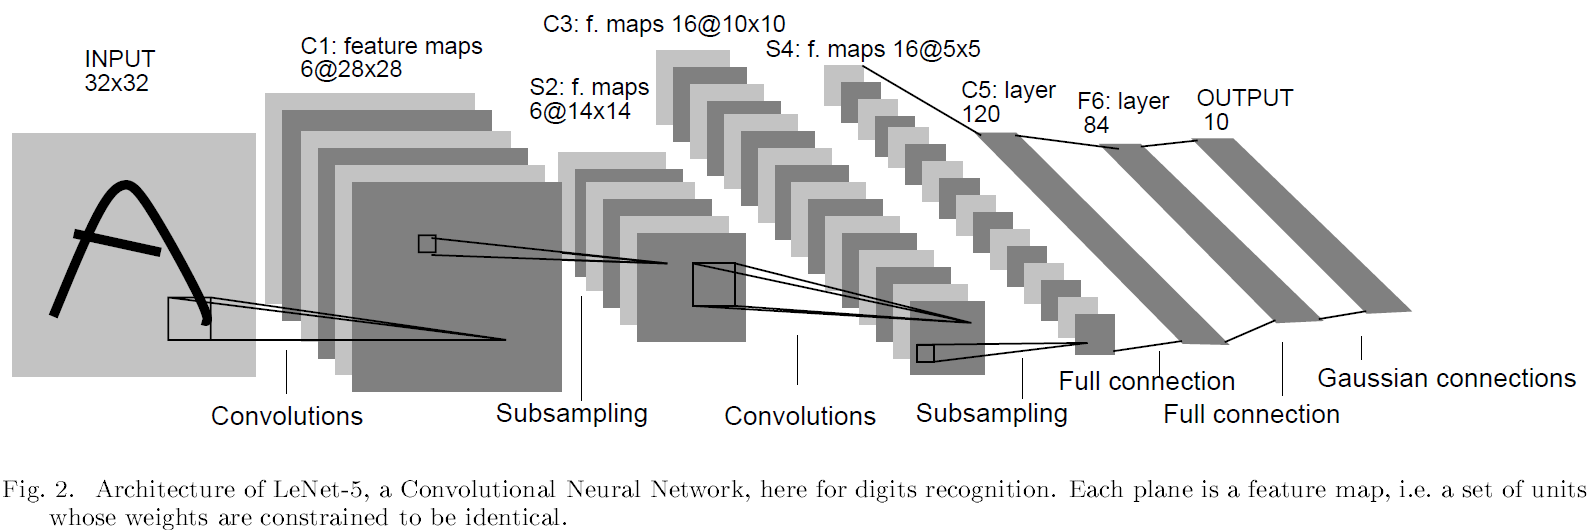
\includegraphics[width=16cm]{images/models/lenet-5.png}
    \label{fig:lenet-5}
\end{figure}

\section{AlexNet}
\begin{figure}[H]
    \centering
    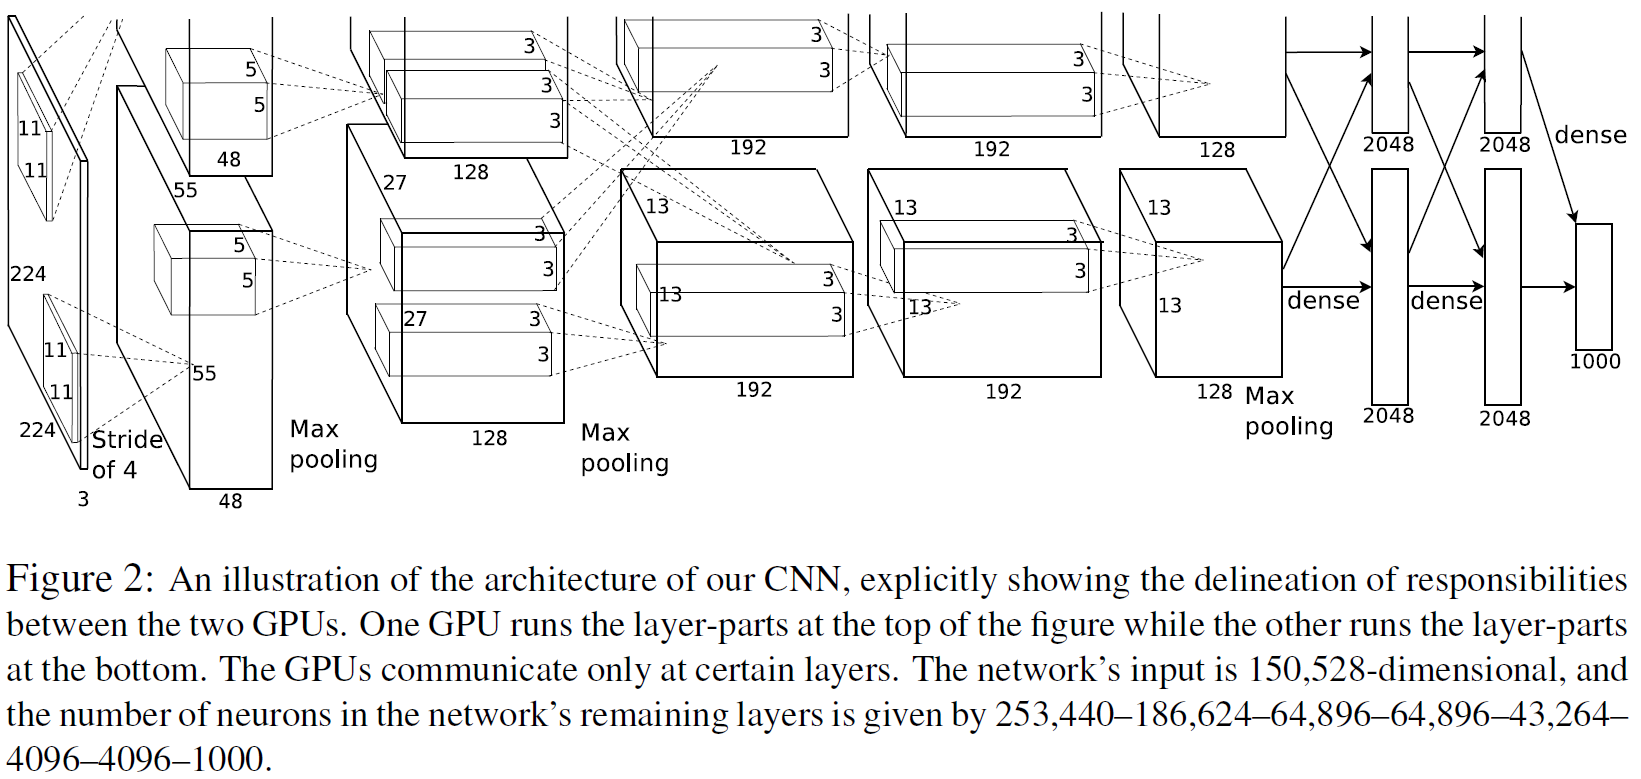
\includegraphics[width=16cm]{images/models/alexnet.png}
    \label{fig:alexnet}
\end{figure}

\section{VGG}
\begin{figure}[H]
    \centering
    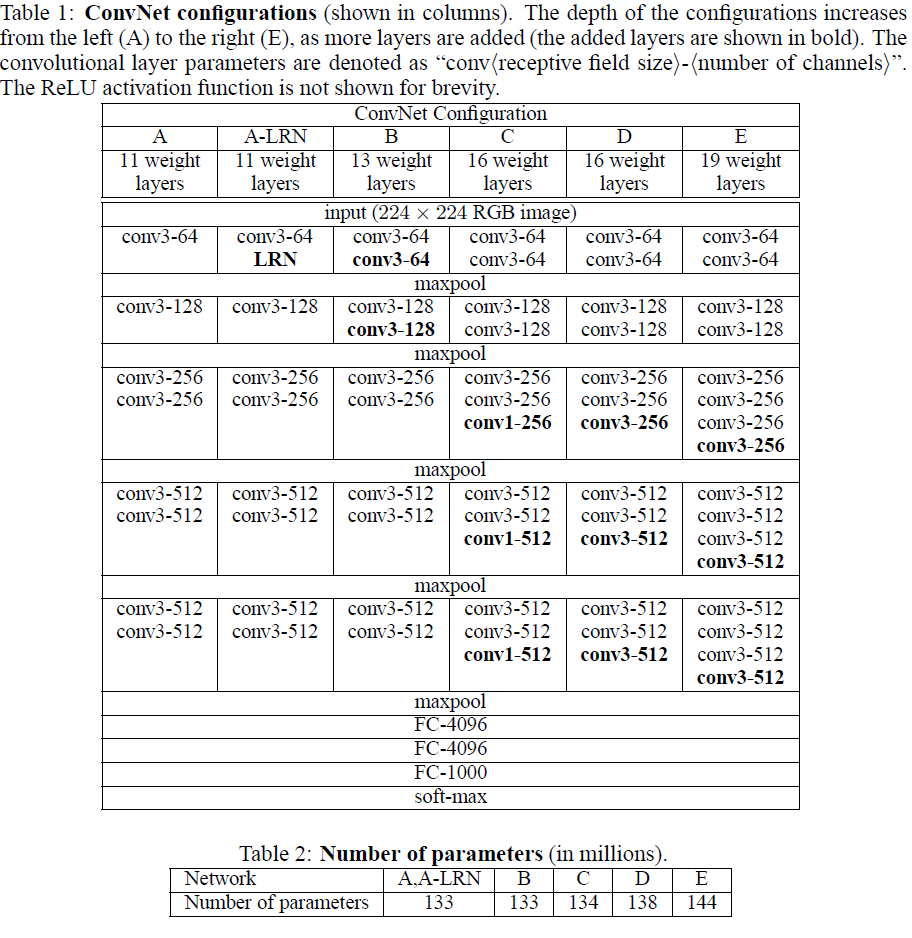
\includegraphics[width=16cm]{images/models/vgg.png}
    \label{fig:vgg}
\end{figure}

\section{GoogLeNet(Inception-v1)}
\subsection{Inception Module}
\begin{figure}[H]
    \centering
    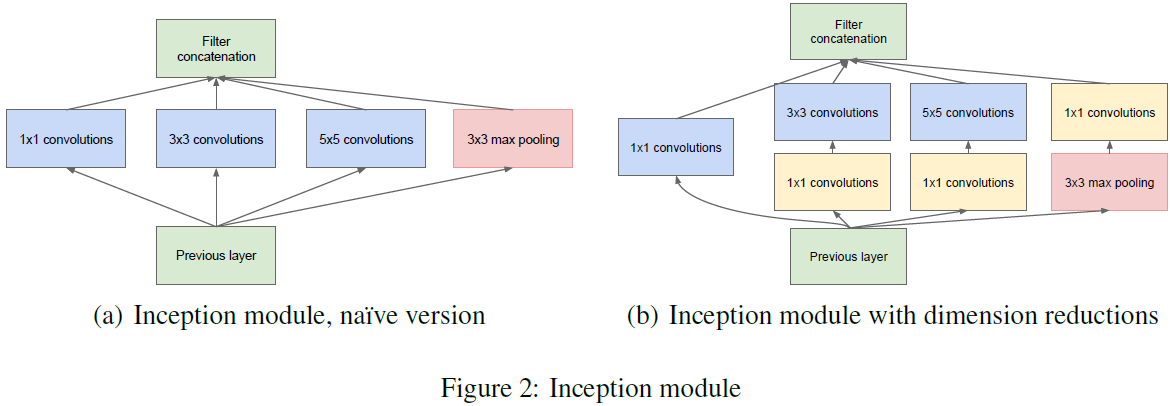
\includegraphics[width=14cm]{images/models/inception_module.png}
    \label{fig:inception_module}
\end{figure}

\subsection{Inception-v1}

\begin{figure}[H]
    \centering
    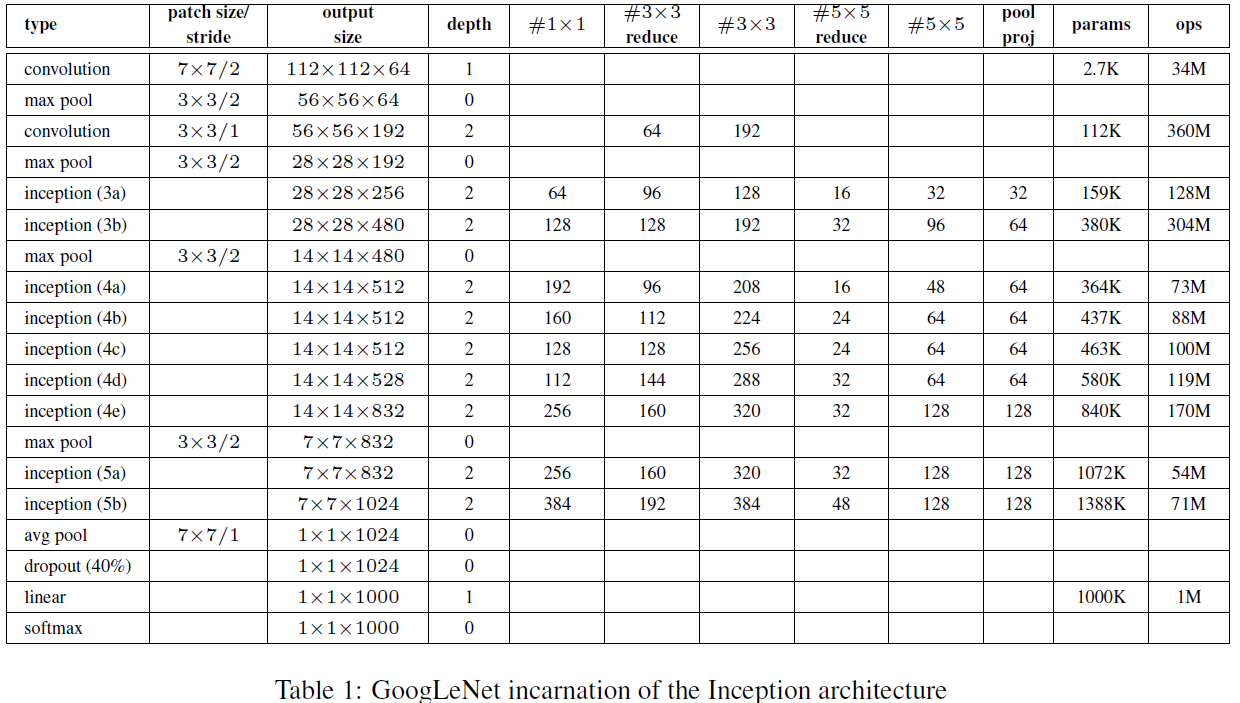
\includegraphics[width=16cm]{images/models/googlenet.png}
    \label{fig:googlenet}
\end{figure}

\begin{figure}[H]
    \centering
    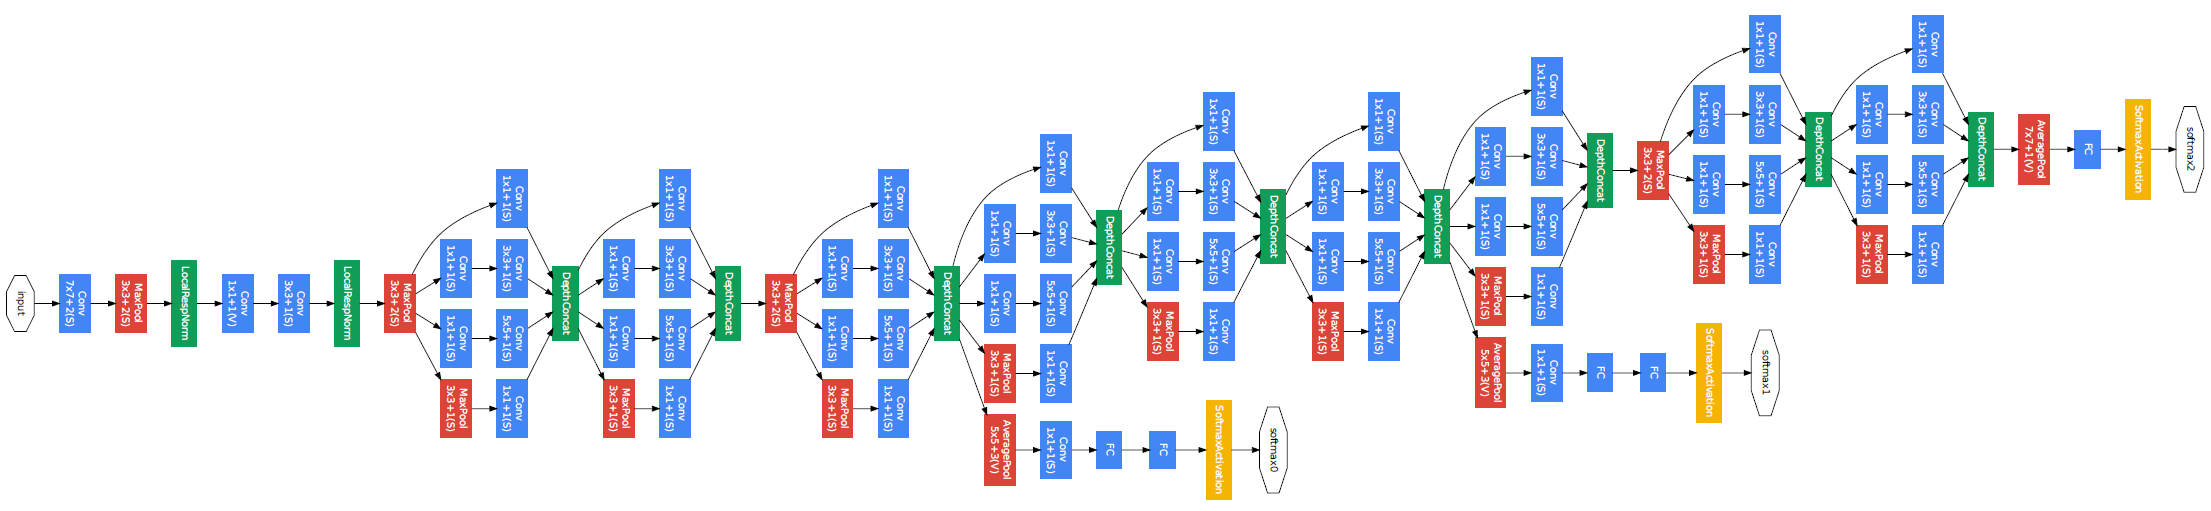
\includegraphics[width=16cm]{images/models/googlenet_arch.png}
    \label{fig:googlenet_arch}
\end{figure}

\section{ResNets}
\subsection{Residual Block}
\begin{figure}[H]
    \centering
    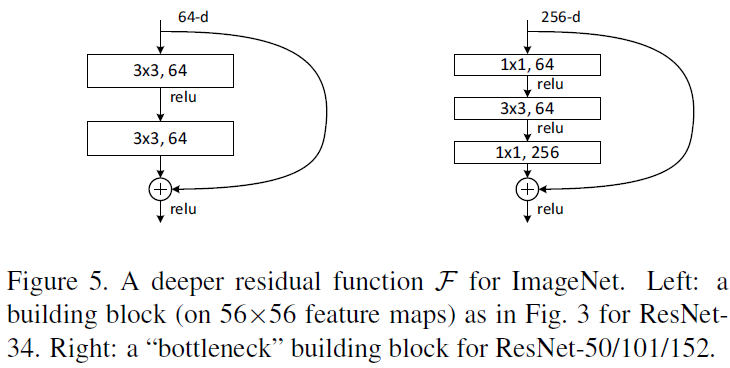
\includegraphics[width=8cm]{images/models/residualblock.png}
    \label{fig:residualblock}
\end{figure}

\subsection{ResNets}
\begin{figure}[H]
    \centering
    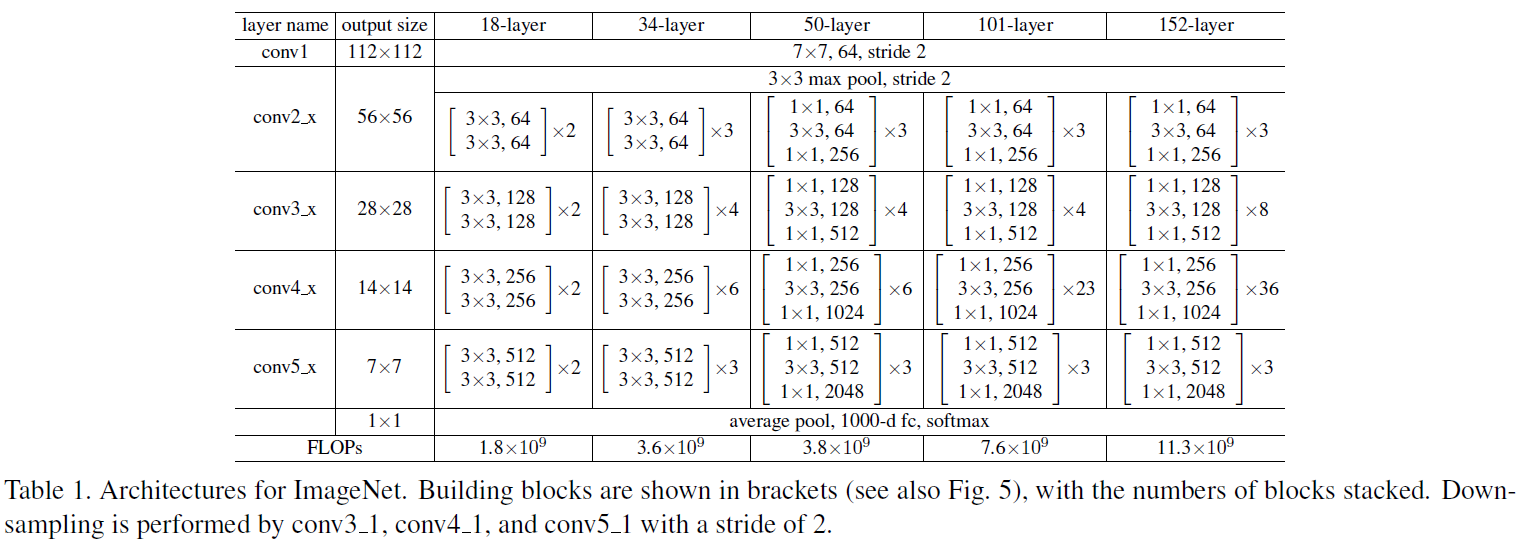
\includegraphics[width=16cm]{images/models/resnets.png}
    \label{fig:resnets}
\end{figure}
\begin{figure}[H]
    \centering
    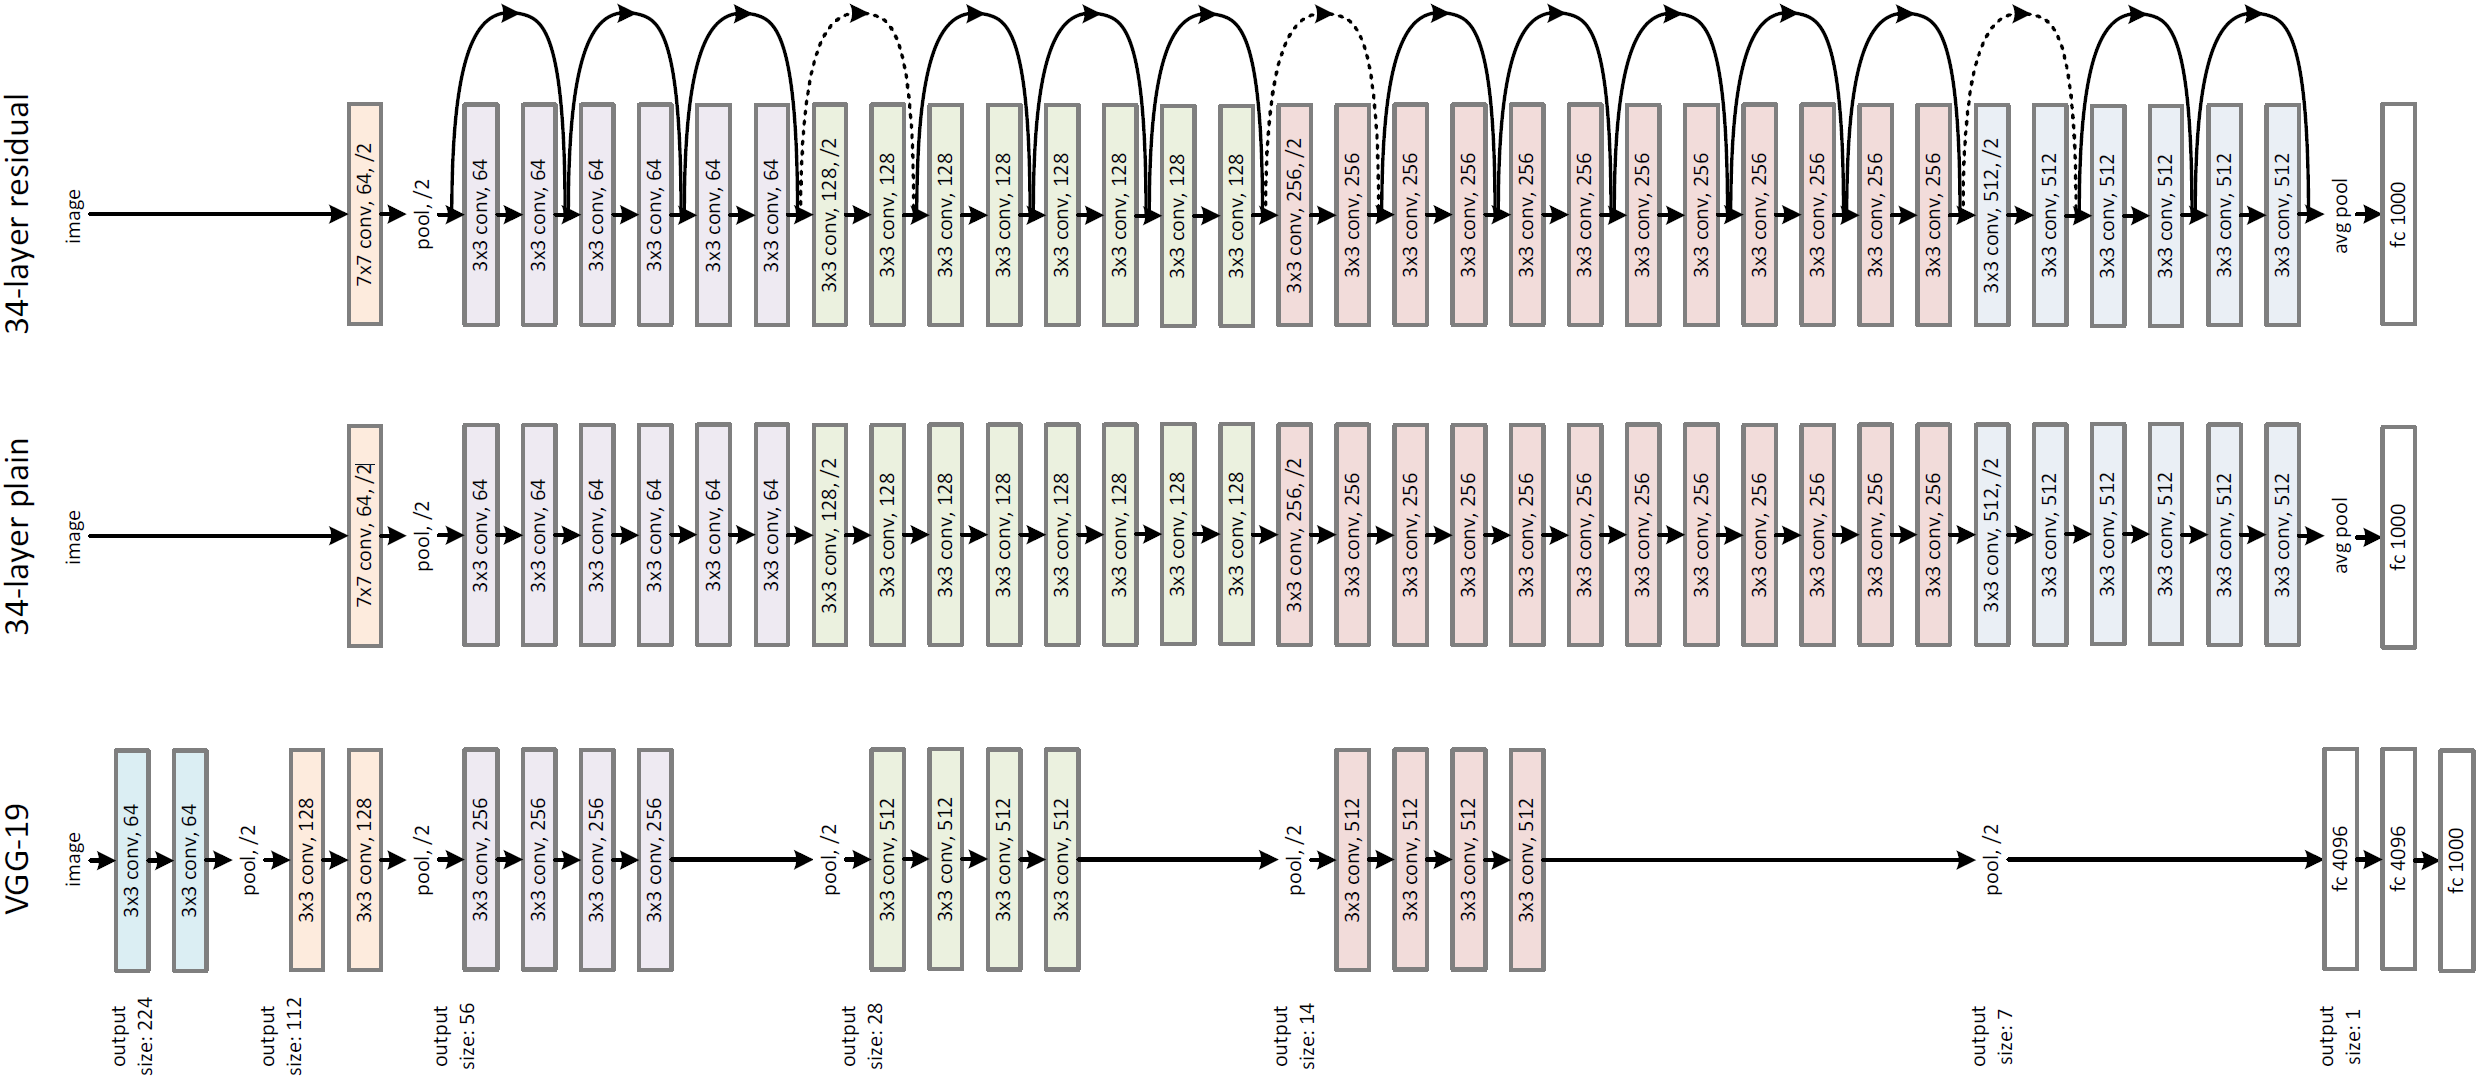
\includegraphics[width=16cm]{images/models/resnets_arch.png}
    \label{fig:resnets_arch}
\end{figure}

\section{Inception-v2, Inception-v3}
\subsection{General Design Principles}
\begin{itemize}
    \item Avoid representational bottlenecks, especially early in the network.
    \item Higher dimensional representations are easier to process locally within a network.
    \item Spatial aggregation can be done over lower dimensional embeddings without much or any loss in representational power.
    \item Balance the width and depth of the network.
\end{itemize}

\subsection{Inception Modules}

\begin{figure}[htbp]
    \centering

    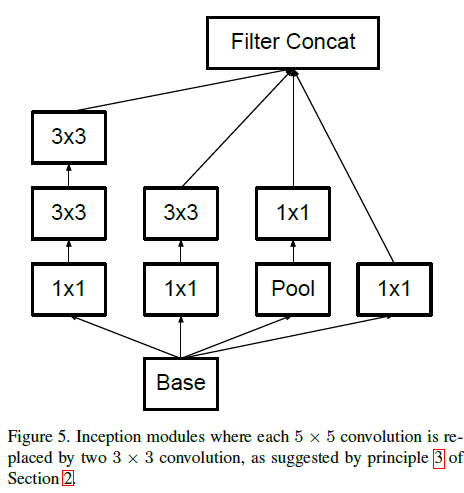
\includegraphics[width=6cm]{images/models/inception_m1.png}
    \hspace{1in}
    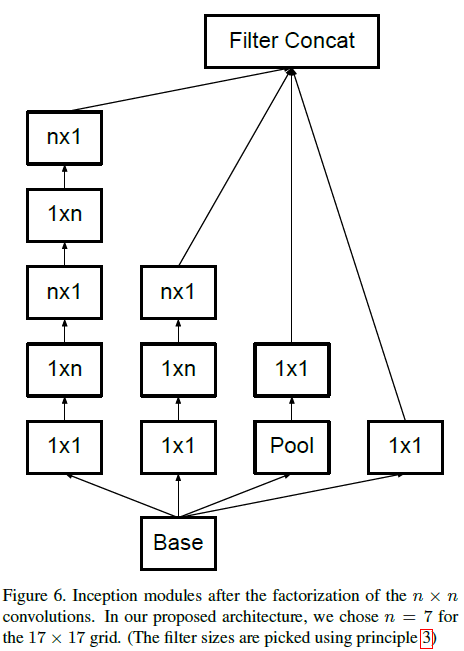
\includegraphics[width=6cm]{images/models/inception_m2.png}
    \hspace{1in}
    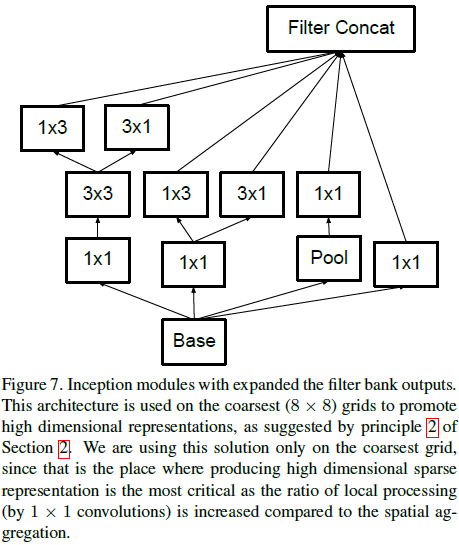
\includegraphics[width=6cm]{images/models/inception_m3.png}
    \hspace{1in}
    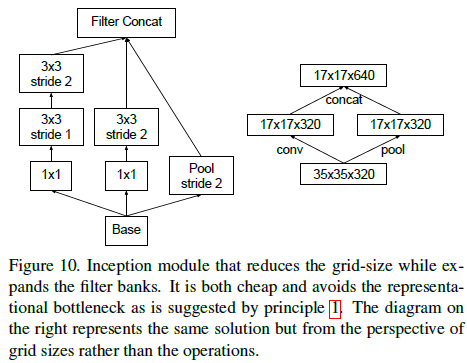
\includegraphics[width=6cm]{images/models/inception_m4.png}
    \caption{Inception Modules}
\end{figure}

\subsection{Inception-v2}
\begin{figure}[H]
    \centering
    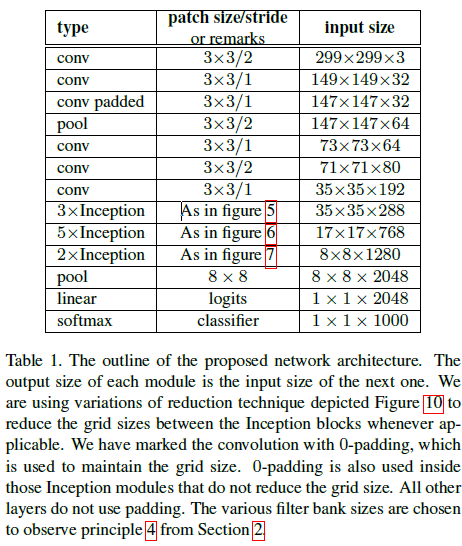
\includegraphics[width=8cm]{images/models/inception_v2v3.png}
    \label{fig:inception_v2v3}
\end{figure}

\subsection{Inception-v3}
\begin{itemize}
    \item RMSProp Optimizer.
    \item Factorized 7x7 convolutions.
    \item BatchNorm in the Auxillary Classifiers.
    \item Label Smoothing
\end{itemize}

\section{Inception-v4, Inception-ResNet}

\section{Xception}
\begin{quotation}
    We present an interpretation of Inception modules 
as being an intermediate step in-between regular convolution
and the depthwise separable convolution operation. In this
light, a depthwise separable convolution can be understood
as an Inception module with a maximally large number of towers.
\end{quotation}

\subsection{Xception Module}
\begin{figure}[H]
    \centering
    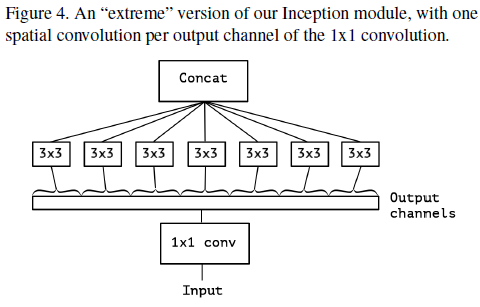
\includegraphics[width=8cm]{images/models/xception_m.png}
    \label{fig:xception_m}
\end{figure}

\subsection{Xception}
\begin{figure}[H]
    \centering
    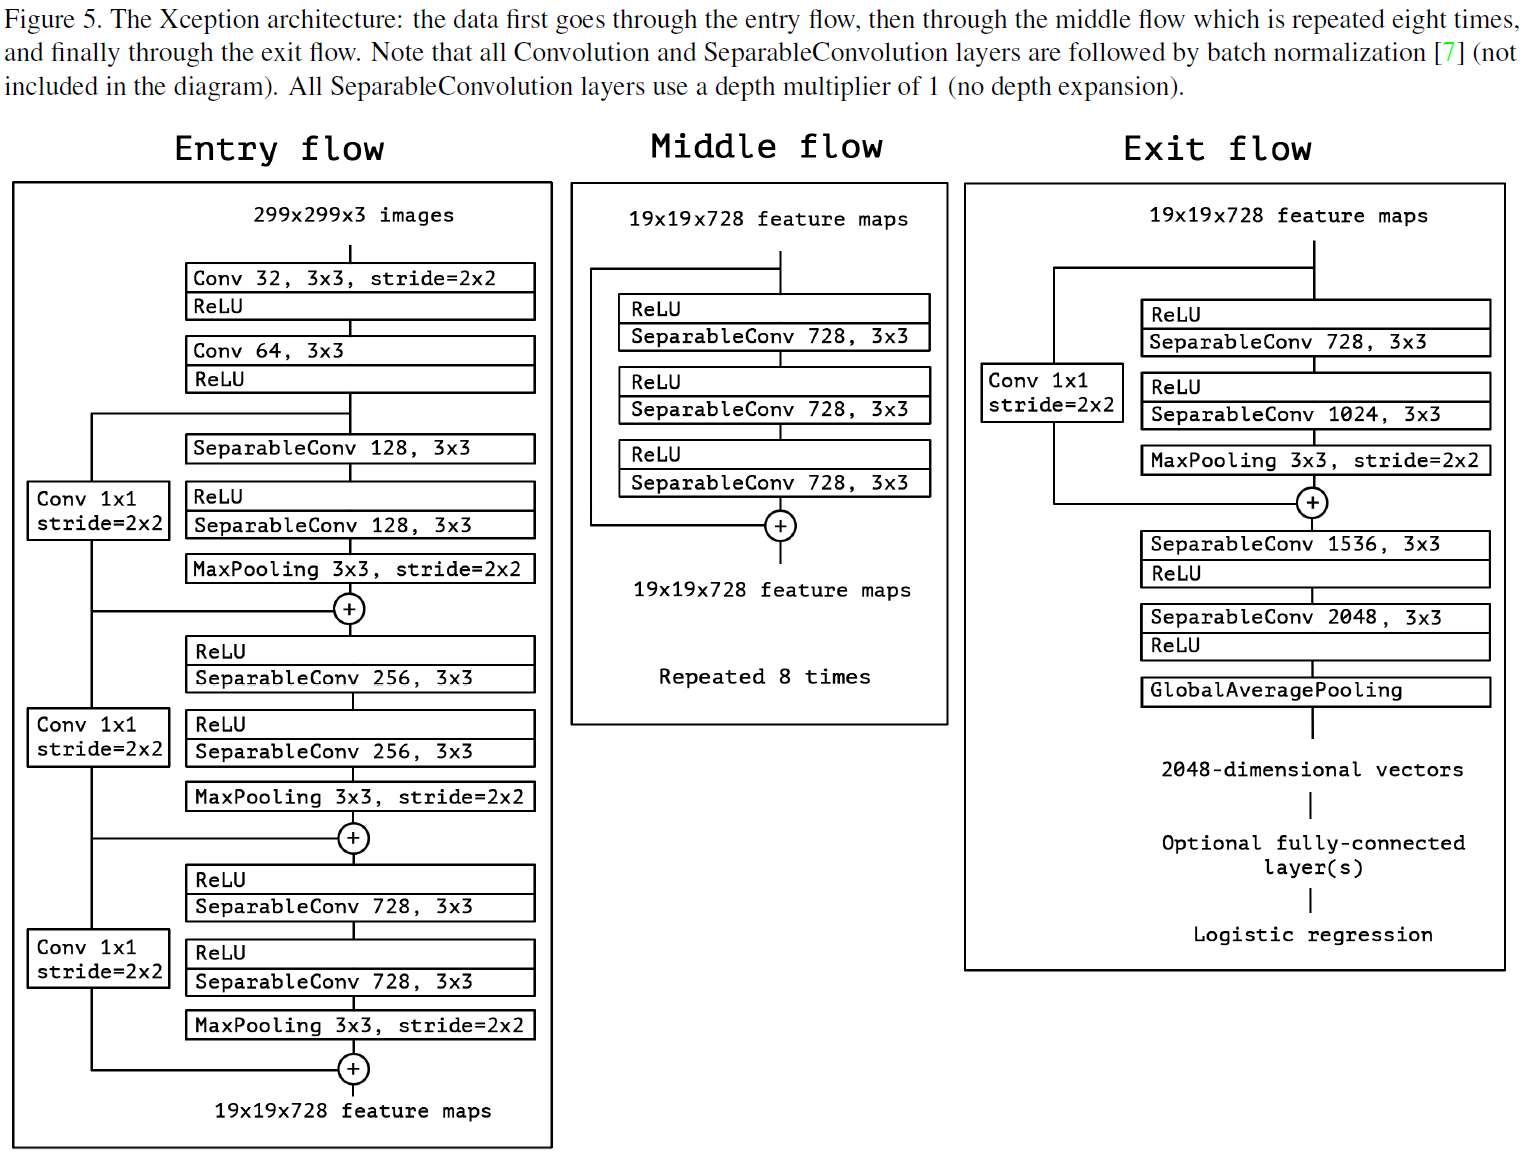
\includegraphics[width=16cm]{images/models/xception.png}
    \label{fig:xception}
\end{figure}

\section{ResNeXt}
Group Convolution + Skip connection

\subsection{ResNeXt Block}
\begin{figure}[H]
    \centering
    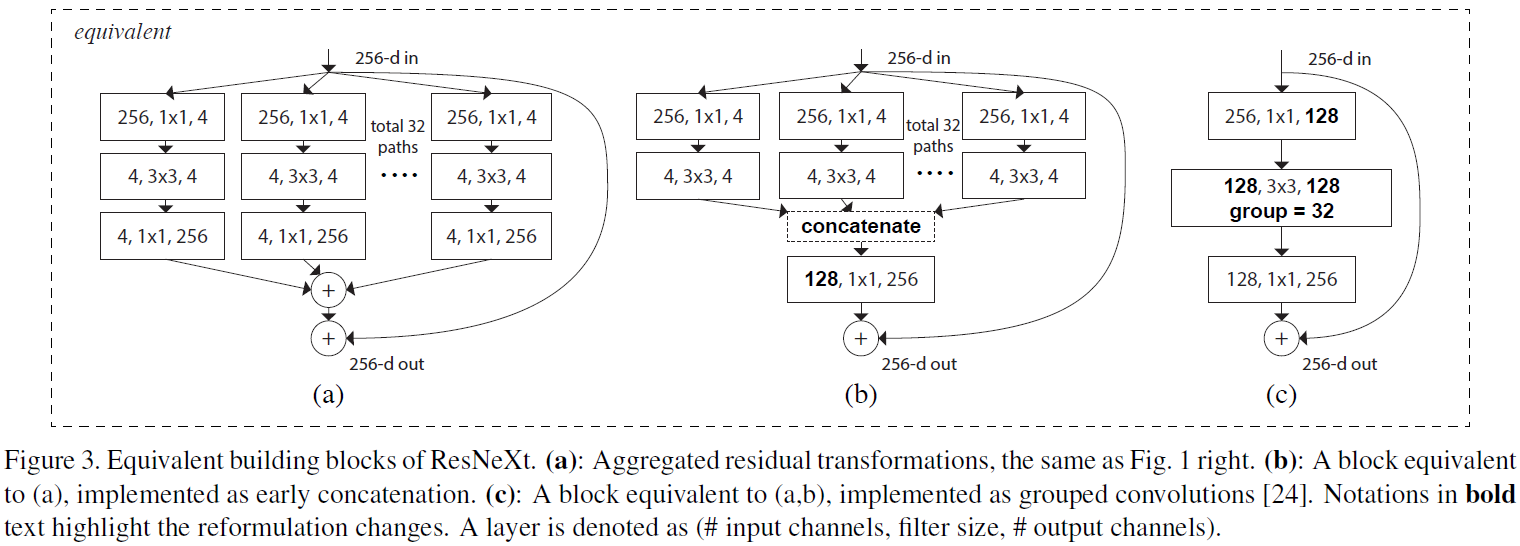
\includegraphics[width=16cm]{images/models/resnext_blocks.png}
    \label{fig:resnext_blocks}
\end{figure}

\subsection{ResNeXt}
\begin{figure}[H]
    \centering
    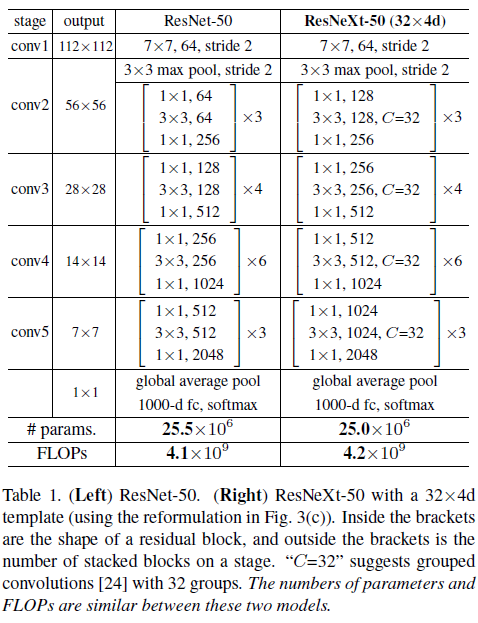
\includegraphics[width=8cm]{images/models/resnext.png}
    \label{fig:resnext}
\end{figure}

\section{MobileNets}

\subsection{Depthwise Separable Convolution}
\begin{figure}[H]
    \centering
    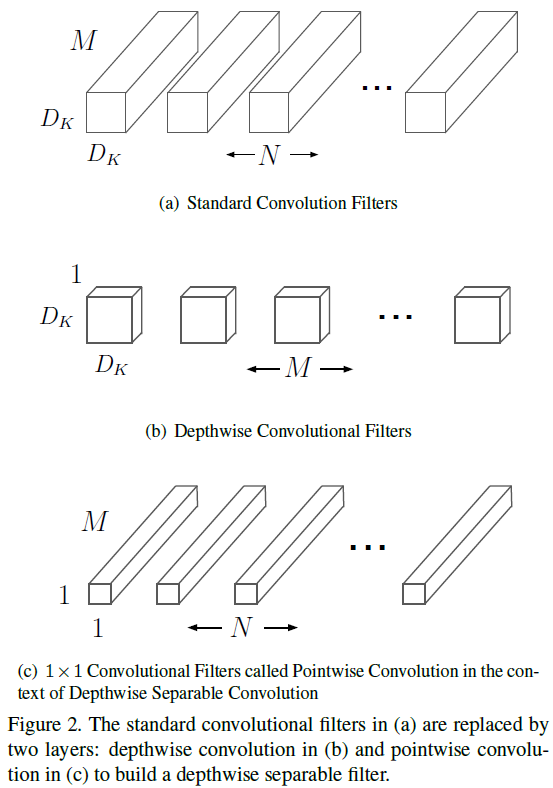
\includegraphics[width=8cm]{images/models/depthwise_separable_conv.png}
    \label{fig:depthwise_separable_conv}
\end{figure}

\subsection{MobileNets}
\begin{figure}[H]
    \centering
    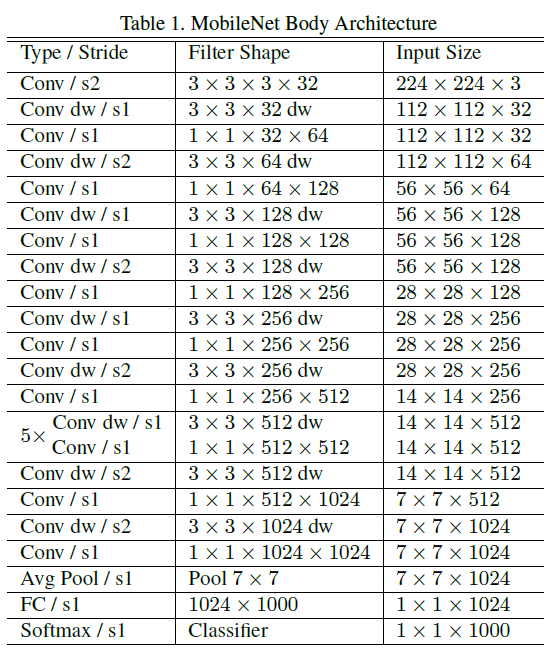
\includegraphics[width=8cm]{images/models/mobilenets.png}
    \label{fig:mobilenets}
\end{figure}

\section{ShuffleNet}
\subsection{Channel Shuffle}
\begin{figure}[H]
    \centering
    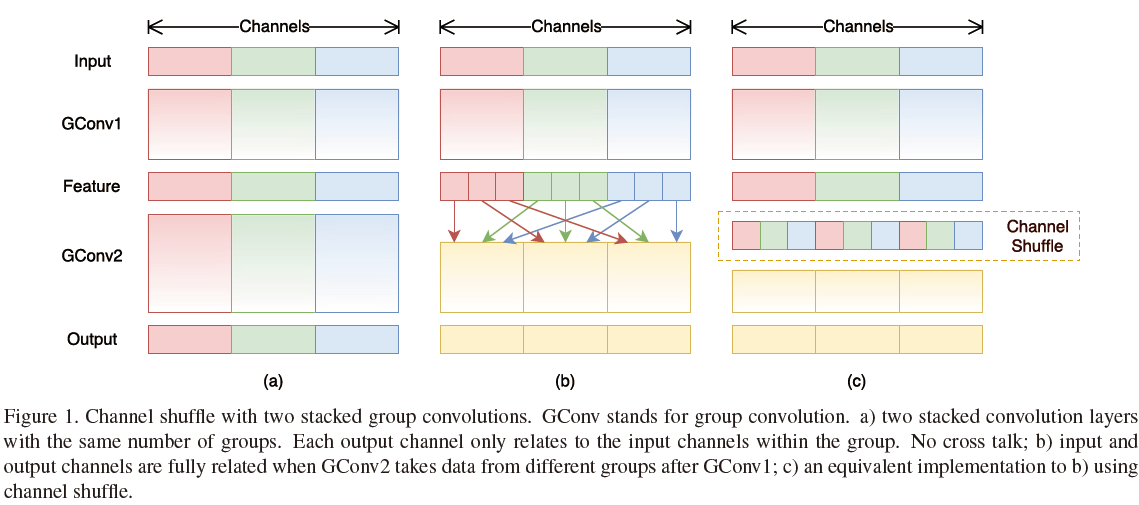
\includegraphics[width=16cm]{images/models/channel_shuffle.png}
    \label{fig:channel_shuffle}
\end{figure}

\subsection{ShuffleNet Unit}
\begin{figure}[H]
    \centering
    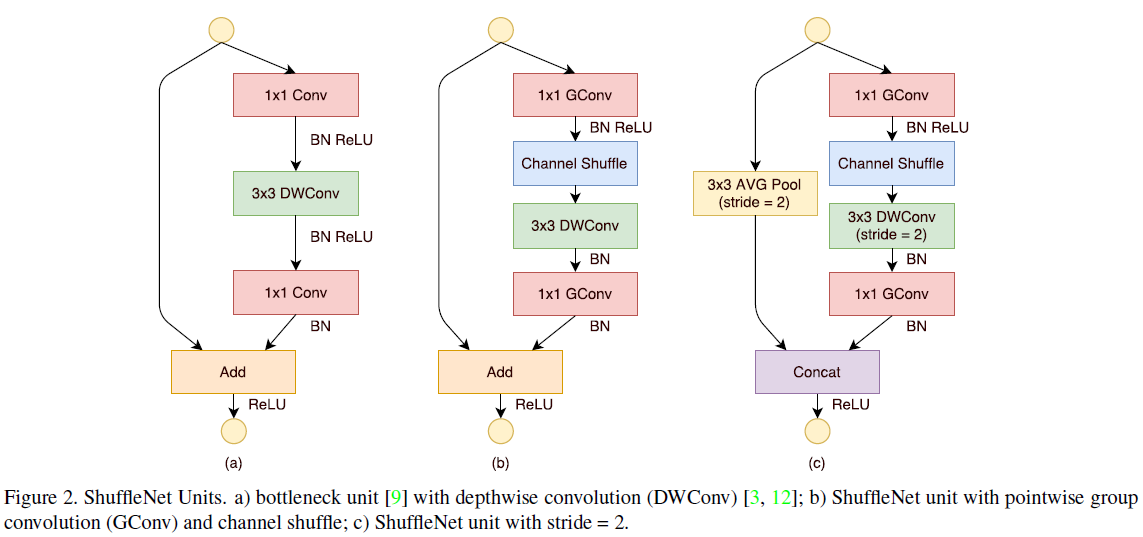
\includegraphics[width=16cm]{images/models/shufflenet_unit.png}
    \label{fig:shufflenet_unit}
\end{figure}

\subsection{ShuffleNet}
\begin{figure}[H]
    \centering
    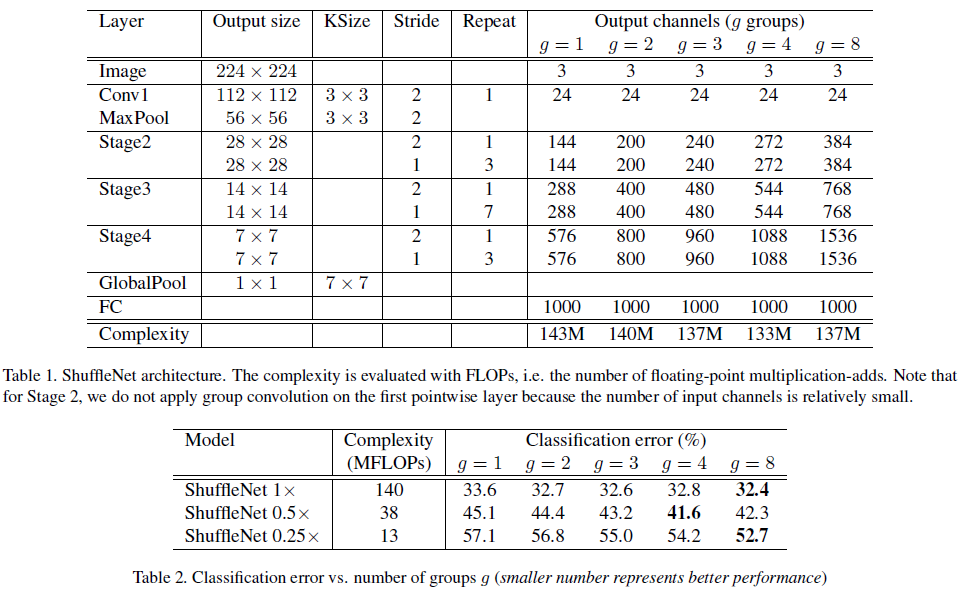
\includegraphics[width=16cm]{images/models/shufflenet.png}
    \label{fig:shufflenet}
\end{figure}

\section{MobileNetv2}

\subsection{Bottleneck residual block}

\begin{figure}[H]
    \centering
    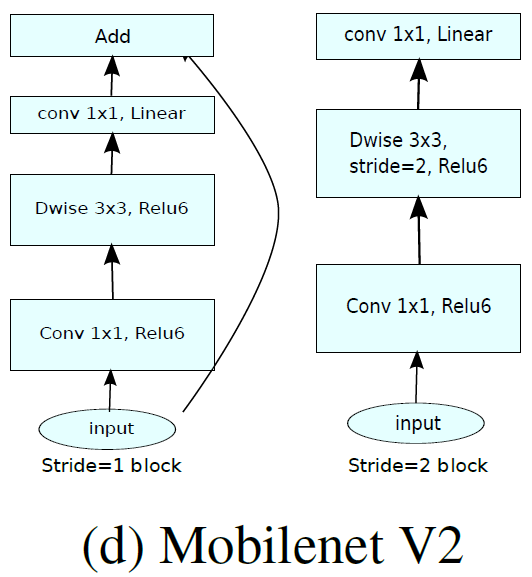
\includegraphics[width=6cm]{images/models/mobilenetv2_block.png}
    \label{fig:mobilenetv2_block}
\end{figure}

\begin{figure}[H]
    \centering
    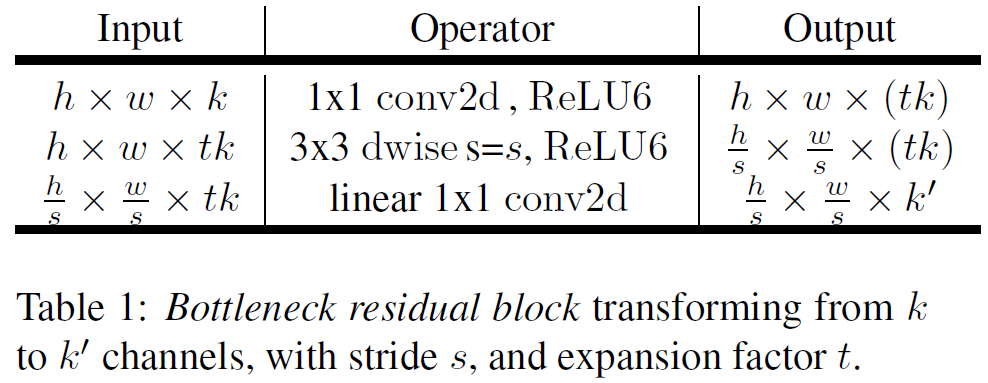
\includegraphics[width=8cm]{images/models/bottleneck_residual_block.png}
    \label{fig:bottleneck_residual_block}
\end{figure}

\subsection{MobileNetv2}
\begin{figure}[H]
    \centering
    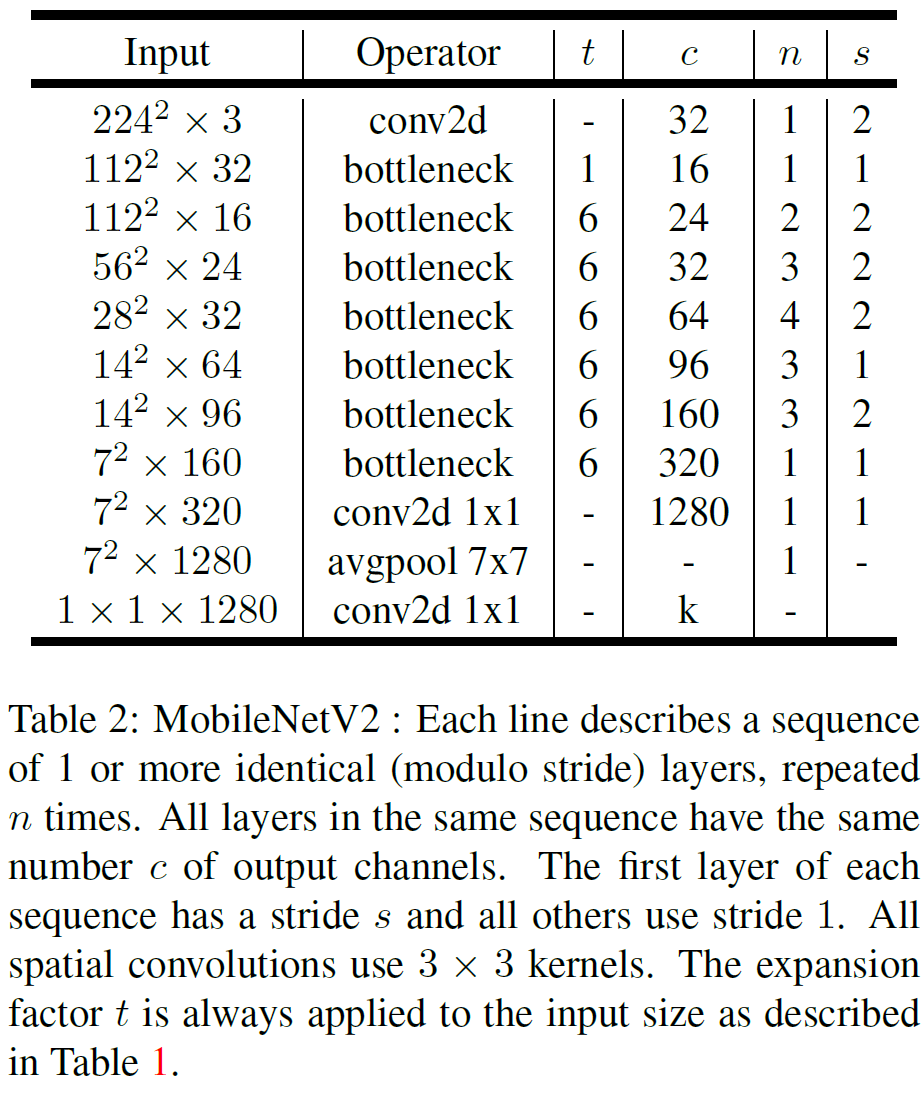
\includegraphics[width=8cm]{images/models/mobilenetv2.png}
    \label{fig:mobilenetv2}
\end{figure}

\section{ShuffleNetv2}
\subsection{ShuffleNetv2 Blocks}
\begin{figure}[H]
    \centering
    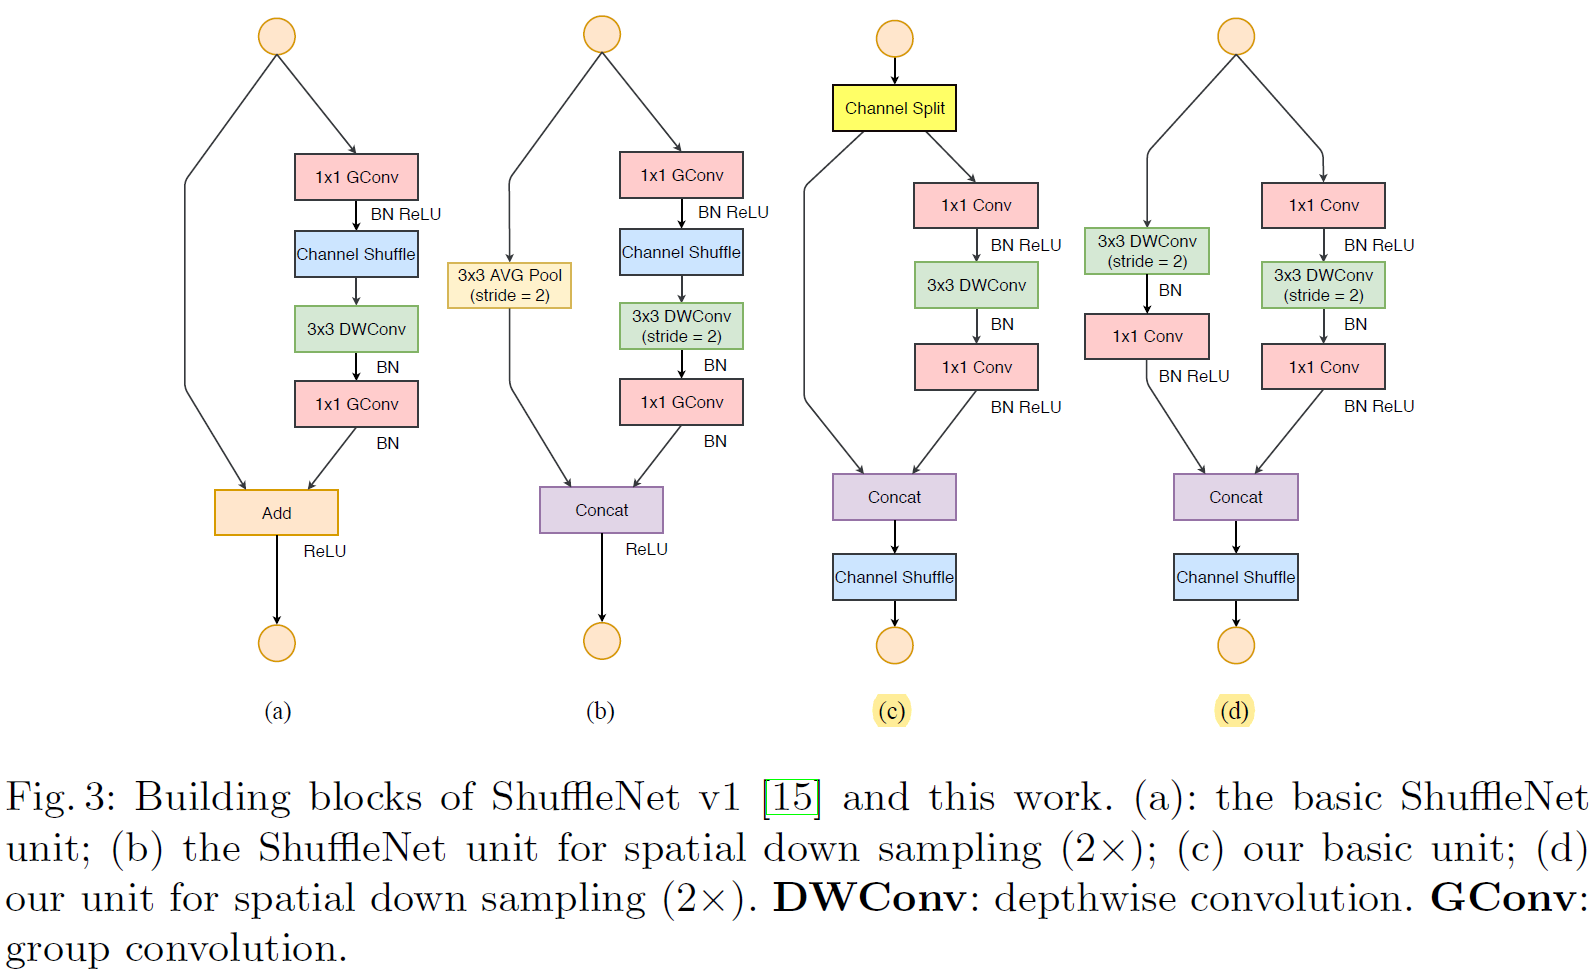
\includegraphics[width=8cm]{images/models/shufflenetv2_block.png}
    \label{fig:shufflenetv2_block}
\end{figure}

\subsection{ShuffleNetv2}
\begin{figure}[H]
    \centering
    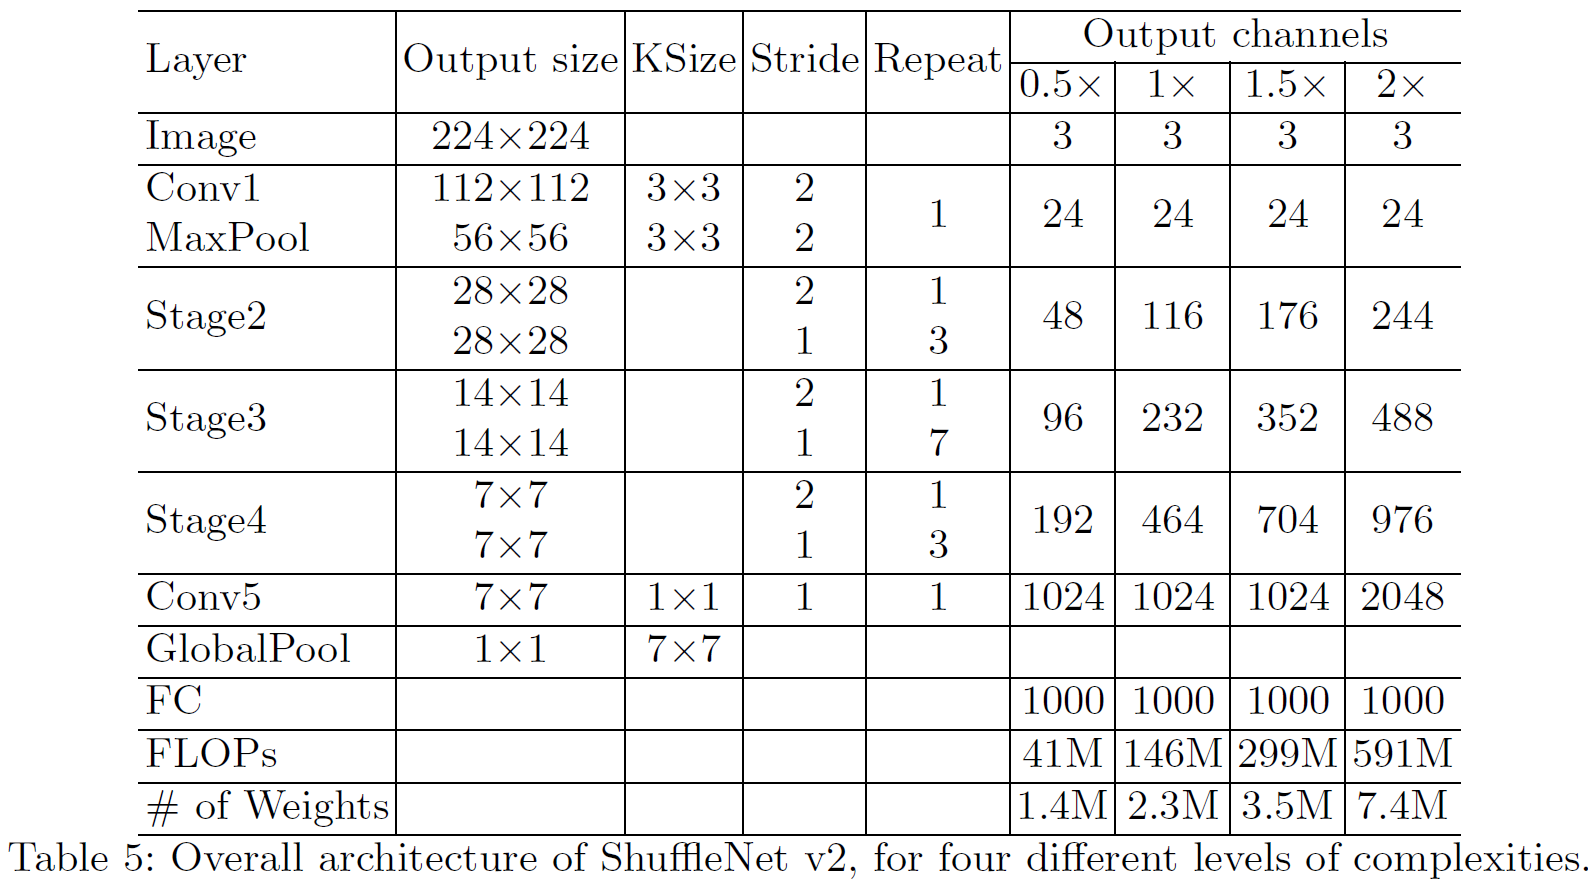
\includegraphics[width=8cm]{images/models/shufflenetv2.png}
    \label{fig:shufflenetv2}
\end{figure}

\subsection{Results}
\begin{figure}[H]
    \centering
    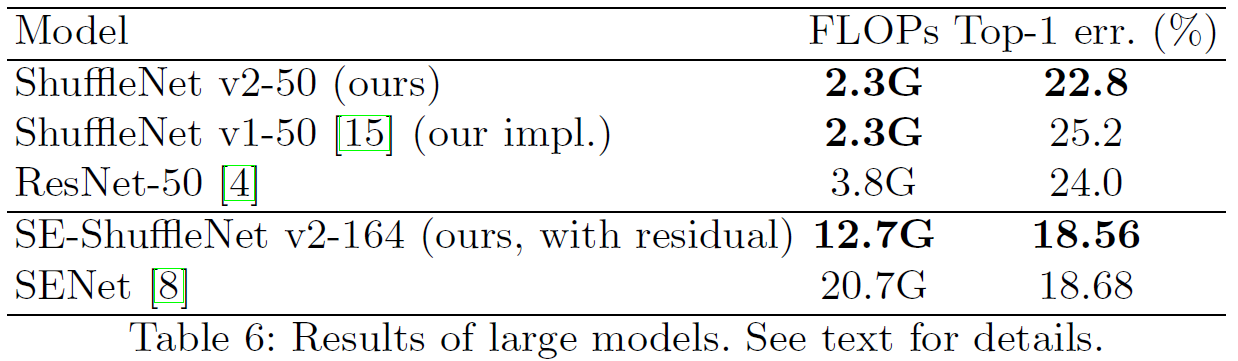
\includegraphics[width=8cm]{images/models/shufflenetv2_res.png}
    \label{fig:shufflenetv2_res}
\end{figure}